\begin{frame}{Margit Sandemo, 1924--2018}
    \note{\tiny{
    The person behind the book series is the renowned novelist \emph{Margit Sandemo}.
    Here's Margit at the book signing event for the re-translation of \emph{Álagafjötrar} held at Eymundsson in 2007.
    A book that began the epic journey of the cursed family we're exploring today.

    \begin{itemize}
    \item Margit Sandemo was born in 1924 and lived a remarkable life until her passing in 2018 at the age of 94—her journey intersected with our ÍSKISUR project.
    \item As a Norwegian-Swedish author, her literary impact in the Nordic countries is undeniable and enduring.
    \item Her father, a Norwegian poet, bequeathed her a literary lineage. Furthermore, she intriguingly claimed lineage to a Nobel Prize-winning author through an alleged affair.
    \item Although surrounded by literature, Margit embarked on her authorial journey at 40, a testament to the adage, 'it's never too late.'
    \item From the 1980s onwards, her novels consistently graced the best-seller lists in the Nordics, showcasing her unparalleled storytelling.
    \item Among her notable works, three series stand prominent:
        \emph{The Legend of the Ice People} from the 1980s, which is our primary topic for today.
        \emph{The Warlock} in the early 1990s, delving into mystical elements, particularly one witch lineage.
        \emph{The Legend of the Realm of Light} in the late 1990s, following the later generations of the Ice People and their continued struggles against dark forces.
    \item Margit seamlessly integrated history and fiction. Drawing inspiration from her noble Oxenstierna ancestors,
    she weaved them into pivotal historical events like the Thirty Years' War.
    Moreover, her fictional world was populated with mythological elements, with Lucifer finding a home in Dimmuborgir,
    which served not just as a backdrop but also as an inadvertent advertisement for Iceland abroad.
    \emph{Such fusion of history, legacy, and mythology provided her readers with a rich, resonating narrative}.
    \item The Ice People remained her muse for nearly two decades, a testament to her commitment and creativity.
\end{itemize}

}}

    \begin{columns}[T]
        \begin{column}{0.6\textwidth}
            \begin{itemize}
                \item Norwegian-Swedish author
                \item Father was a Norwegian poet, Anders Underdal
                \item Claimed lineage to Nobel Prize-winning author Bjørnstjerne Bjørnson
                \item First published at forty years old
                \item Best-selling author in the Nordic countries since the 1980s
            \end{itemize}
            \vfill
            \begin{scriptsize}
                \begin{table}
                    \begin{tabular}{rcc}
                        \textbf{Notable Book Series}     & \textbf{Years} & $n$ \\ \midrule
                        The Legend of the Ice People     & 1982--89       & 47  \\
                        The Warlock                      & 1991--94       & 15  \\
                        The Legend of the Realm of Light & 1995--99       & 12
                    \end{tabular}
                \end{table}
            \end{scriptsize}
        \end{column}
        \begin{column}{0.4\textwidth}
            \centering
            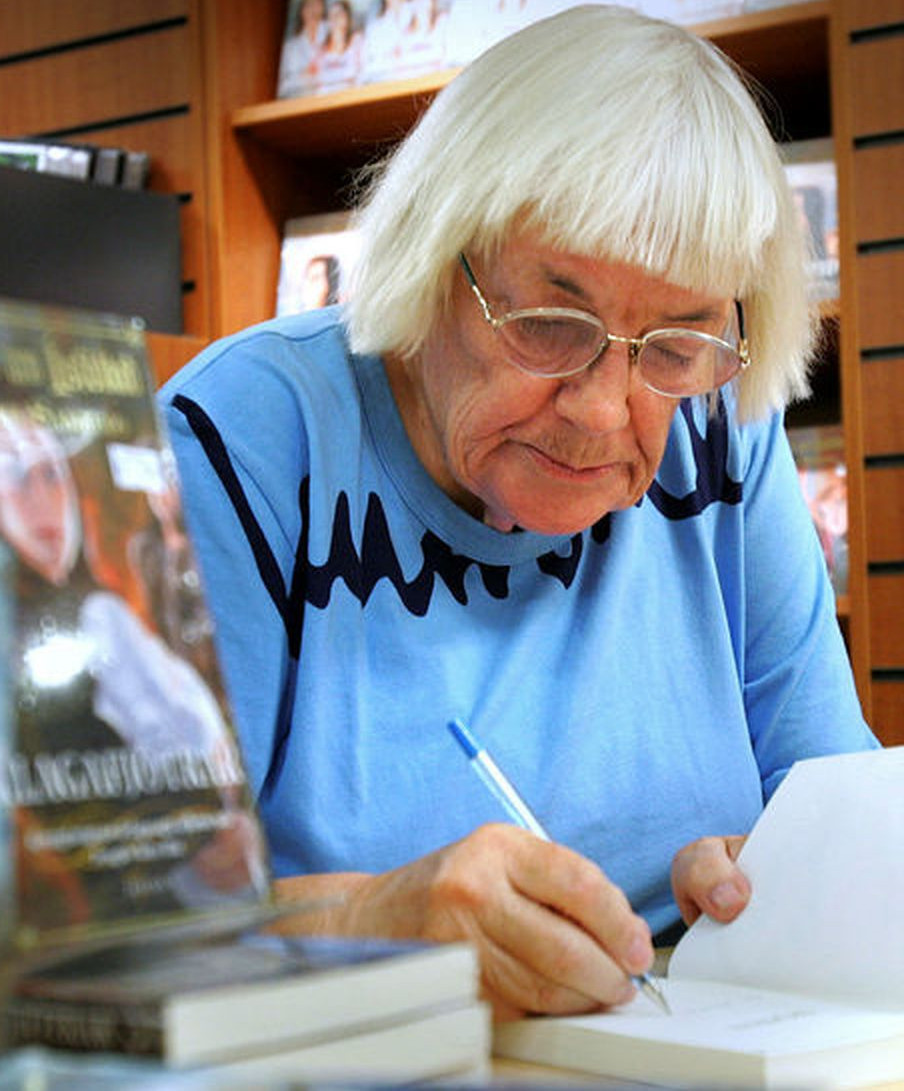
\includegraphics[width=\textwidth]{../rek-data-beers/figures/margit_sandemo}
            \begin{tiny}
                mbl.is/Þorvaldur Örn Kristmundsson
            \end{tiny}

            \vfill
            Margit signing \emph{Álagafjötrar} in Eymundsson, 2007
        \end{column}
    \end{columns}
\end{frame}

\begin{frame}{Publications}

    \note{\scriptsize
        The scatter plot illustrates the timeline of Margit's book publications in Iceland by the publisher \emph{Prenthúsið} over an intense 8-year span.

        Throughout this period, Margit's prolificacy is evident: a remarkable 47 books were published,
        averaging a release every 8-9 weeks, with Tuesdays often being the chosen release day.

        Some discernible patterns from the data:
        \begin{itemize}
            \item Margit had a penchant for consistency, often sticking to a structure of 14 chapters (with few exceptions) for each book.
            \item As the series advanced, a decrease in the length of the books is observed.
            This aligns with her reflections in the final epilogue, \emph{Is There Anybody Out There?} (an homage to Pink Floyd's \emph{The Wall}).
            \item There she discloses her struggle with maintaining the narrative's momentum, hinting at writer's fatigue and the challenge of keeping the saga engaging.
            \item Ingibjörg Jónsdóttir embarked on translating the series in 1982 and faithfully rendered the first 33 books into Icelandic.
            Unfortunately, her life was cut short, passing away on Christmas morning in 1986.
            After Ingibjörg's untimely death, Ingibjörg Briem took on the mantle to complete the translations for the remaining 14 books of the series.
        \end{itemize}



}
    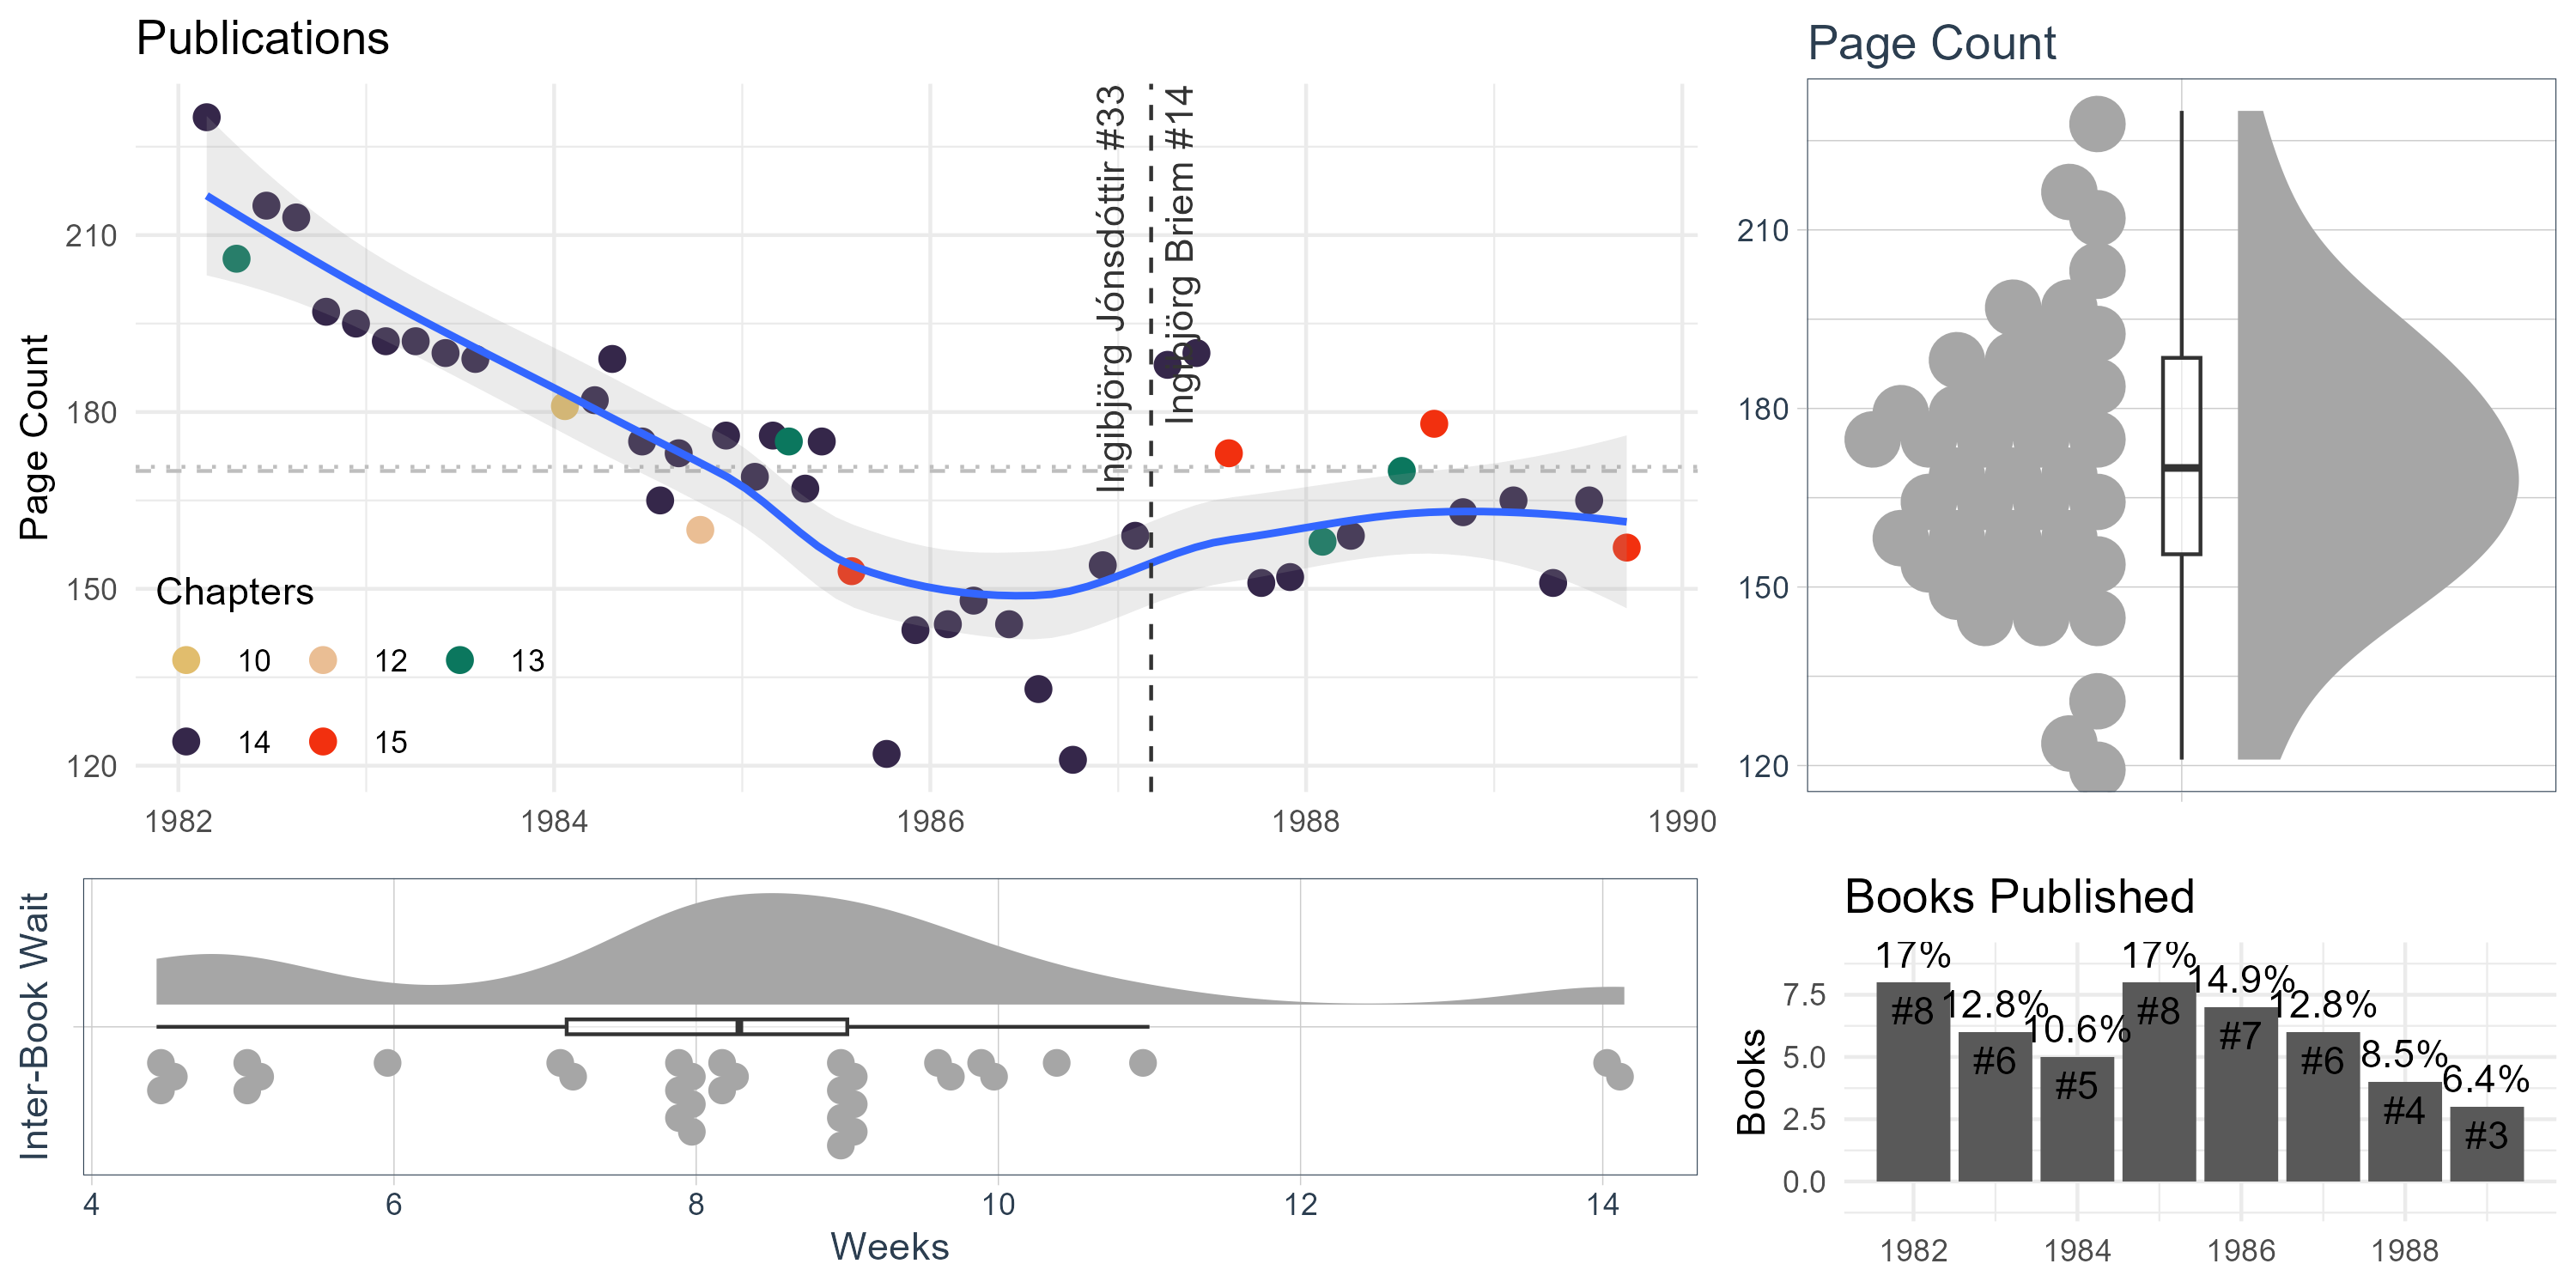
\includegraphics[width=\textwidth]{../rek-data-beers/R/figures/margit_count}
    \vspace{-24pt}
    \begin{itemize}
        \item 47 books, 652 chapters, 8,023 pages, 8 years
        \item Average book length: 170 pages (avg. 13.9 chapters)
        \item Released 1 book every 2 months (avg. 57.9 days), usually on Tue.
    \end{itemize}
\end{frame}
